\documentclass[11pt]{article}

% Latex template from James Richard Forbes, 2025/10/13, McGill University.
% Parts of this template are from Paul Furgal, Timothy D. Barfoot, Christopher J. Damaren, Adam Phillip, and others. 

\usepackage[top=1.0in, bottom=1.0in, left=1.0in, right=1.0in]{geometry}
\usepackage{amsmath} % cmex10
\usepackage{amssymb}
\usepackage{amsthm}
\usepackage{bm}
\usepackage{mathrsfs}
\usepackage{graphicx}
\usepackage{epsfig}
\usepackage{subfigure}
\usepackage{enumerate}
\usepackage{cite}
\usepackage{setspace}
\usepackage{cancel} % To cancel out terms
\usepackage{color}
\usepackage{wrapfig}
\usepackage{xspace}
\usepackage[colorlinks, citecolor=black, linkcolor=black, linktocpage=true]{hyperref}
\usepackage{times}
\usepackage{array}
\usepackage{parskip}
\usepackage{paralist}
\usepackage{titlesec}

% Custom commands
\newcommand{\norm}[1]{\left\Vert#1\right\Vert} % Norm
\newcommand{\p}{\partial}
\newcommand{\f}{\frac}
\newcommand{\dt}{\mathrm{d}t} 
\newcommand{\dee}{\textrm{d}}
\newcommand{\trans}{{\ensuremath{\mathsf{T}}}} % transpose
\newcommand{\trace}{ {\ensuremath{\mathrm{tr}}} } % \trace
\newcommand{\rk}{{\ensuremath{\mathrm{rk}}}} % rank
\newcommand{\onehalf}{\mbox{$\textstyle{\frac{1}{2}}$}} 

% Basic bold for letters and symbols
\DeclareMathAlphabet{\mbf}{OT1}{ptm}{b}{n}
\newcommand{\mbs}[1]{{\boldsymbol{#1}}}
\newcommand{\mbm}[1]{ \textbf{\textit{#1}} } % {\bm #1}
\newcommand{\mbc}[1]{ \boldsymbol{\mathcal{#1}} } 

% Helper bold symbols
\newcommand{\mbsdot}[1]{{\dot{\boldsymbol{#1}}}}
\newcommand{\mbsbar}[1]{{\bar{\boldsymbol{#1}}}}
\newcommand{\mbshat}[1]{{\hat{\boldsymbol{#1}}}}
\newcommand{\mbsdel}[1]{{\delta {\boldsymbol{#1}}}}
\newcommand{\mbstilde}[1]{{\tilde{\boldsymbol{#1}}}}
\newcommand{\mbfdot}[1]{{\dot{\mbf{#1}}}}
\newcommand{\mbfbar}[1]{{\bar{\mbf{#1}}}}
\newcommand{\mbfhat}[1]{{\hat{\mbf{#1}}}}
\newcommand{\mbfdel}[1]{{\delta{\mbf{#1}}}}
\newcommand{\mbftilde}[1]{{\tilde{\mbf{#1}}}}

% Packed lists
\newenvironment{packed_enum}{
\begin{enumerate}
  \setlength{\itemsep}{1pt}
  \setlength{\parskip}{0pt}
  \setlength{\parsep}{0pt}
}{\end{enumerate}}

\newenvironment{packed_itemize}{
\begin{itemize}
  \setlength{\itemsep}{1pt}
  \setlength{\parskip}{0pt}
  \setlength{\parsep}{0pt}
}{\end{itemize}}

% Footer
\usepackage{fancyhdr, lastpage}
\pagestyle{fancy}
\lhead{}
\rhead{} 
\chead{} 
\lfoot{\today}
\cfoot{}
\rfoot{\small Page \thepage\ of \pageref{LastPage}}
\renewcommand{\headrulewidth}{0.0pt} 
\renewcommand{\footrulewidth}{0.75pt}

% Make sure paragraphs indent
\setlength{\parindent}{25pt}


\title{\vfill\textbf{MECH ??? Project Part ?} \\ \textbf{Clever Title} \vfill}

\author{FirstName1 LastName1, Student ID \\ FirstName2 LastName2, Student ID  \\  FirstName3 LastName3, Student ID \\ \small{Department of Mechanical Engineering, McGill University} \\ \small{817 Sherbrooke Street West, Montreal, QC, H3A 0C3}}

\date{\today}

\begin{document}

\begin{titlepage}
\pagenumbering{gobble} % Turns page numbering off for title page
\maketitle
\vfill
\end{titlepage}

\clearpage % new page

\pagenumbering{arabic}
\section{Introduction}
\label{sec:intro}

In the introduction, you introduce the problem, provide motivation, etc. Notice, you can reference sections with a label. A label is like a variable name. For example, this is Section~\ref{sec:intro}.

\subsection{A Subsection}

This is a subsection. Say you want to make a numbered list. Here's how you to it. 

\begin{enumerate}

\item I wanted to get this done \ldots 

\item \ldots and this \ldots

\end{enumerate}

Say you want to make a bulleted list. Here's how you do it. 

\begin{itemize}

\item Here' something \ldots

\item Solving $\mbf{A} \mbf{x} = \mbf{b}$.

\item Solve for this \ldots

\end{itemize}

This list is really spread out. You can make a packed list, like this. 

\begin{packed_itemize}

\item Root-finding.

\item Solving $\mbf{A} \mbf{x} = \mbf{b}$.

\item Solving ODEs. 

\end{packed_itemize}


\section{Writing Math}

Linear equations, such as
\begin{align}
	y & = m x , \label{eq:slope} \\
	\mbf{A} \mbf{x} & = \mbf{b} , \nonumber
\end{align}
satisfy superposition and scaling. Equation~\eqref{eq:slope} is from grade-school. Notice that
\begin{align}
	\mbs{\Xi} \mbfdot{q} = \mbf{0} , 
	\label{eq:nullspace}
\end{align}
meaning $\mbfdot{q}$ lies in the null space of $\mbs{\Xi}$. In \eqref{eq:nullspace} the matrix $\mbs{\Xi}$ does not have full column rank. 

If you want to write an equation without a number, you can write
\begin{align*}
	m \ddot{q}(t) + k q(t) = 0 ,
\end{align*}
which is the equation of a homogenous, second order, ODE. 

You can reference papers and books using bibtex. For example, in \cite{paper_Zanetti_Majji_Bishop_Morari_2009} is discussed state estimation. In the textbook \cite{book_guzzella} and course notes \cite{notes_francis_ECE311} is discussed control. 

Depending on our IDE (e.g., TeXShop vs VS Considerations), you must manually compile as follows: latex bibtex latex latex. 


\section{Making a Table}
A table is shown in Table~\ref{tab:table_example}.

\begin{table}[h]
\caption{This is a table example. Put numbers in a table.}
\label{tab:table_example}
\vspace{5pt}  % add some vertical space.
\begin{center}
\begin{tabular}{|c|c|}
\hline
Left & Right \\
\hline
1 & 2 \\
3 & 4 \\
\hline
\end{tabular}
\end{center}
\label{default}
\end{table}%

\newpage
\section{Making Figures}

Other things, like how to make a figure. For example, Figure~\ref{fig:low_e_equatorial_orbit} is a figure on its own. 

\begin{figure}[ht]
	\centering
        		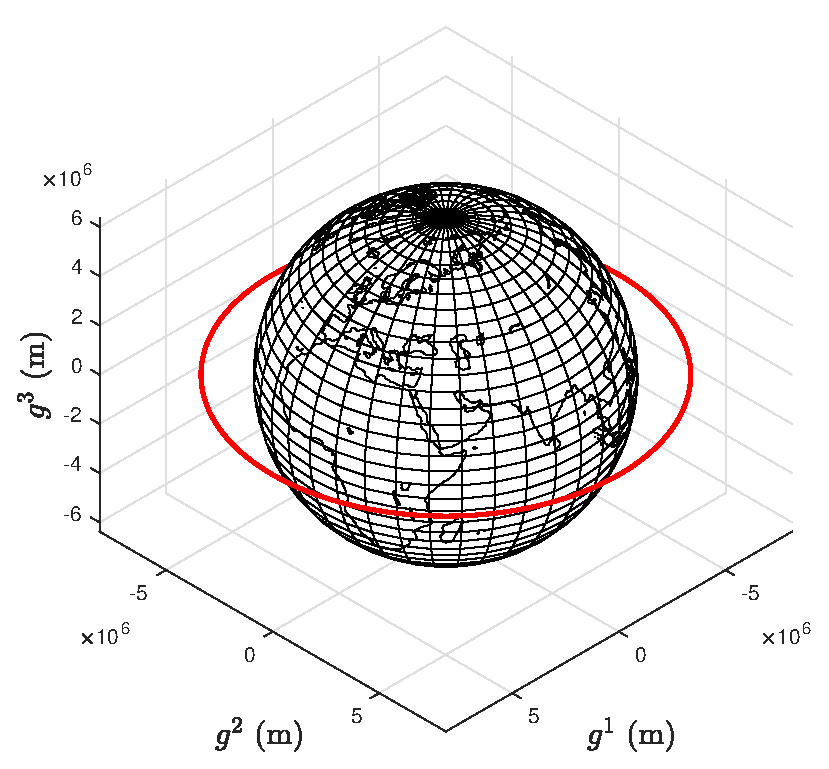
\includegraphics[width=0.5\textwidth]{figs/low_e_equatorial_orbit.eps}
    	\caption{Low eccentricity, equatorial orbit.}
    	\label{fig:low_e_equatorial_orbit}
\end{figure}

On the other hand, Figure~\ref{fig:orbits} has two subfigures, that being Figure~\ref{fig:med_e_polar_orbit} and Figure~\ref{fig:high_e_45_deg_orbit}. Notice how labels are used to reference figures properly. 
\begin{figure}[ht!]
  \centering
  	\subfigure[Medium eccentricity, polar orbit.]{\label{fig:med_e_polar_orbit}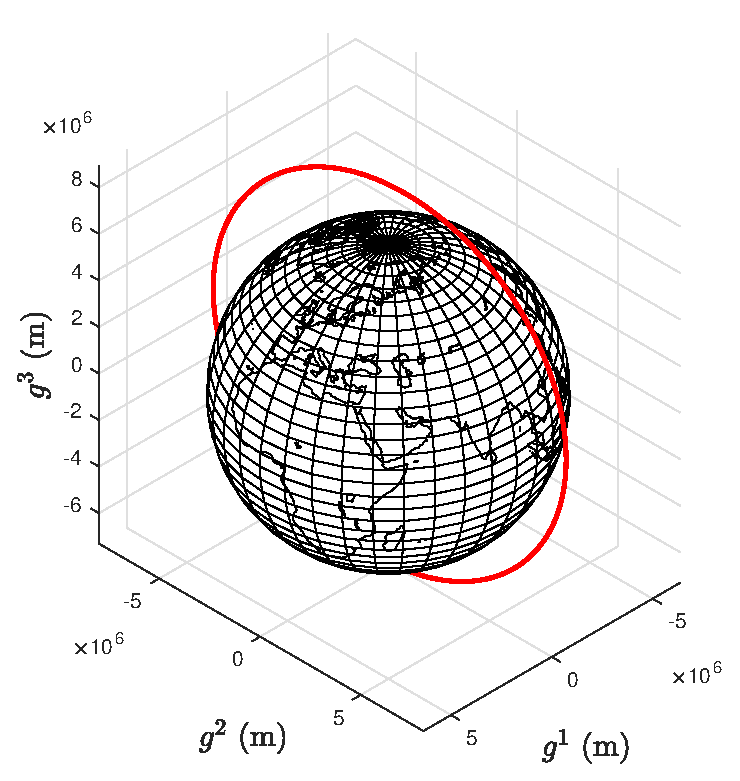
\includegraphics[width=0.375\textwidth]{figs/med_e_polar_orbit.eps}}
	\subfigure[High eccentricity, inclined orbit.]{\label{fig:high_e_45_deg_orbit}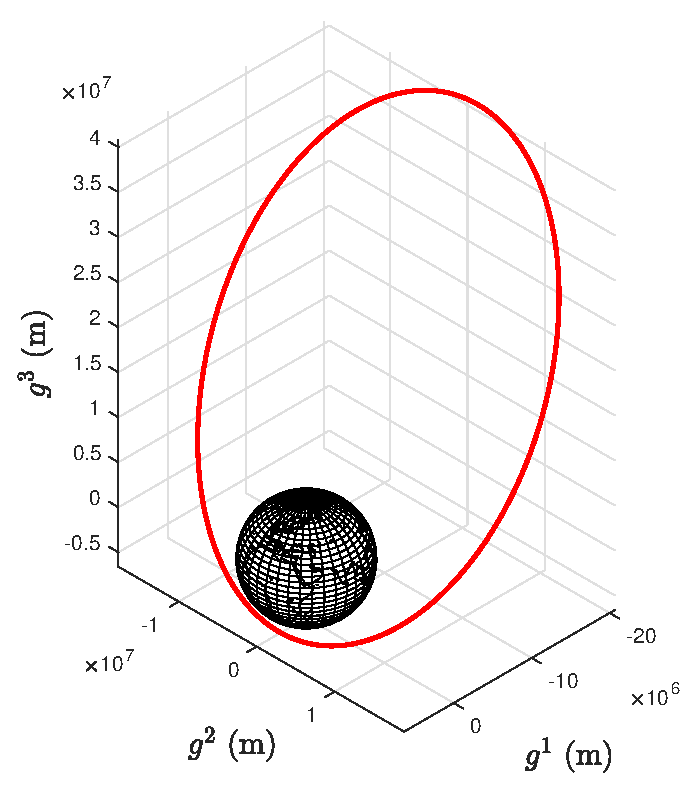
\includegraphics[width=0.375\textwidth]{figs/high_e_45_deg_orbit.eps}}
	\caption{Different kinds of spacecraft orbits around the Earth.}
  \label{fig:orbits}
\end{figure}




\newpage

\addcontentsline{toc}{section}{References}
\bibliographystyle{ieeetr}
\bibliography{references}

\end{document}